\section{The Mythical Man-Month}
The titular chapter explains the guiding principle, and most difficult trap of large-system programming.  the man-month is a unit of measurement for productivity.  In perfectly partitionable tasks, like reaping crops, one can estimate that the quantity produced is the number of men times the number of months they work times some constant.  That is, $Quantity(Units) = N(Men) \times M(Months) \times C \frac{Units}{Man-Months}$, or efficiency remains constant with an increasing number of men.  A graph demonstrating this principle is shown in figure \ref{fig:ideal}  In some cases like assembling cars on a factory line, we may even expect efficiency to increase with number of men because of specialization.

\begin{figure}
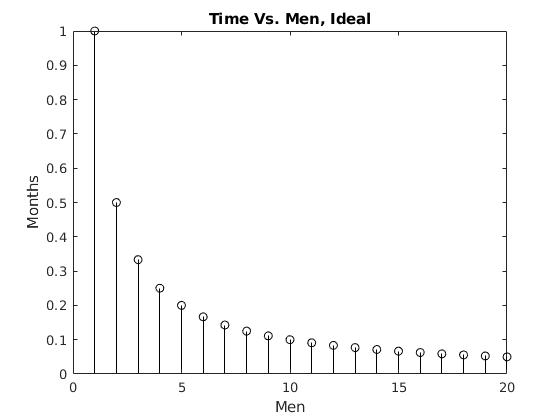
\includegraphics[width=8cm]{idealmanmonth}
\centering
\caption{Time to produce a given quantity versus number of men, perfectly partitionable.  Plot adapted from ``The Mythical Man-Month''}
\label{fig:ideal}
\end{figure}

On the opposite end of the spectrum some tasks are not partionable at all, e.g. the bearing of a child will take nine months no matter how many workers are assigned.  This type of task follows the formula $Quantity(Units) = M(months) \times C \frac{Units}{Month}$  A graph demonstrating this principle is shown in figure \ref{fig:bad}.

\begin{figure}
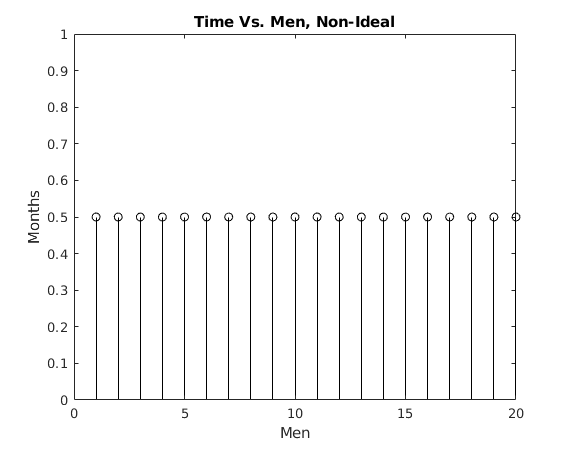
\includegraphics[width=8cm]{badmanmonth}
\centering
\caption{Time to produce a given quantity versus number of men, unpartitionable.  Plot adapted from ``The Mythical Man-Month''}
\label{fig:bad}
\end{figure}

Finally, for complex tasks like large-system programming, the heavy burden of intercommunication is added.  If we assume that every worker must communicate with every other worker in order to complete their tasks, the time cost grows quadratically with the number of men, or $M(months) = C\frac{Man-Months}{Unit}\times\frac{Quanitity(Units)}{N(men)} + B\frac{Months}{Men^2} \times (N(Men))^2$  A graph demonstrating this principle is shown in figure \ref{fig:real}

\begin{figure}
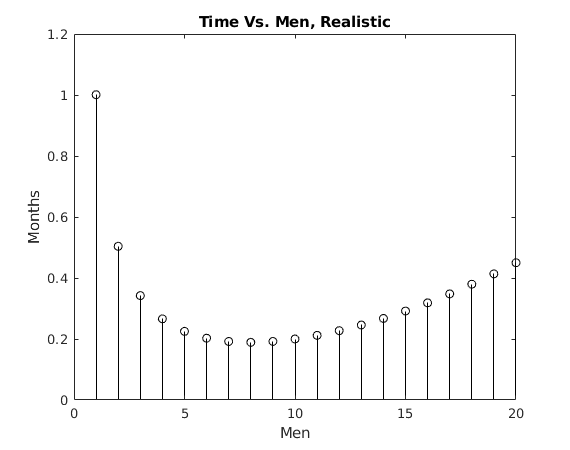
\includegraphics[width=8cm]{realmanmonth}
\centering
\caption{Time to produce a given quantity versus number of men, semi-partitionable.  Plot adapted from ``The Mythical Man-Month''}
\label{fig:real}
\end{figure}

Brooks suggests the following rule of thumb for completing a software task:\\
\vbox{
\begin{itemize}
\setlength\itemsep{0.1em}
\item[] 1/4 planning
\item[] 1/6 coding
\item[] 1/4 component test and early system test
\item[] 1/4 system test, all components in hand
\end{itemize}
}
Brooks claims that, compared to conventional scheduling, more time is devoted to planning, much more time is devoted to testing, and much less time is devoted to actual coding, or implementation.  Brooks says that failure to allow enough time for system testing is particularly disasterous since it is at the end of the schedule, and the software mmay be crucial in supporting other business efforts like shipping new computers.  All of this gives rise to the infamous Brooks's Law: ``Adding manpower to a late software project makes it later.''\
